\section{Backend Architecture}

\begin{figure}[H]
\centering
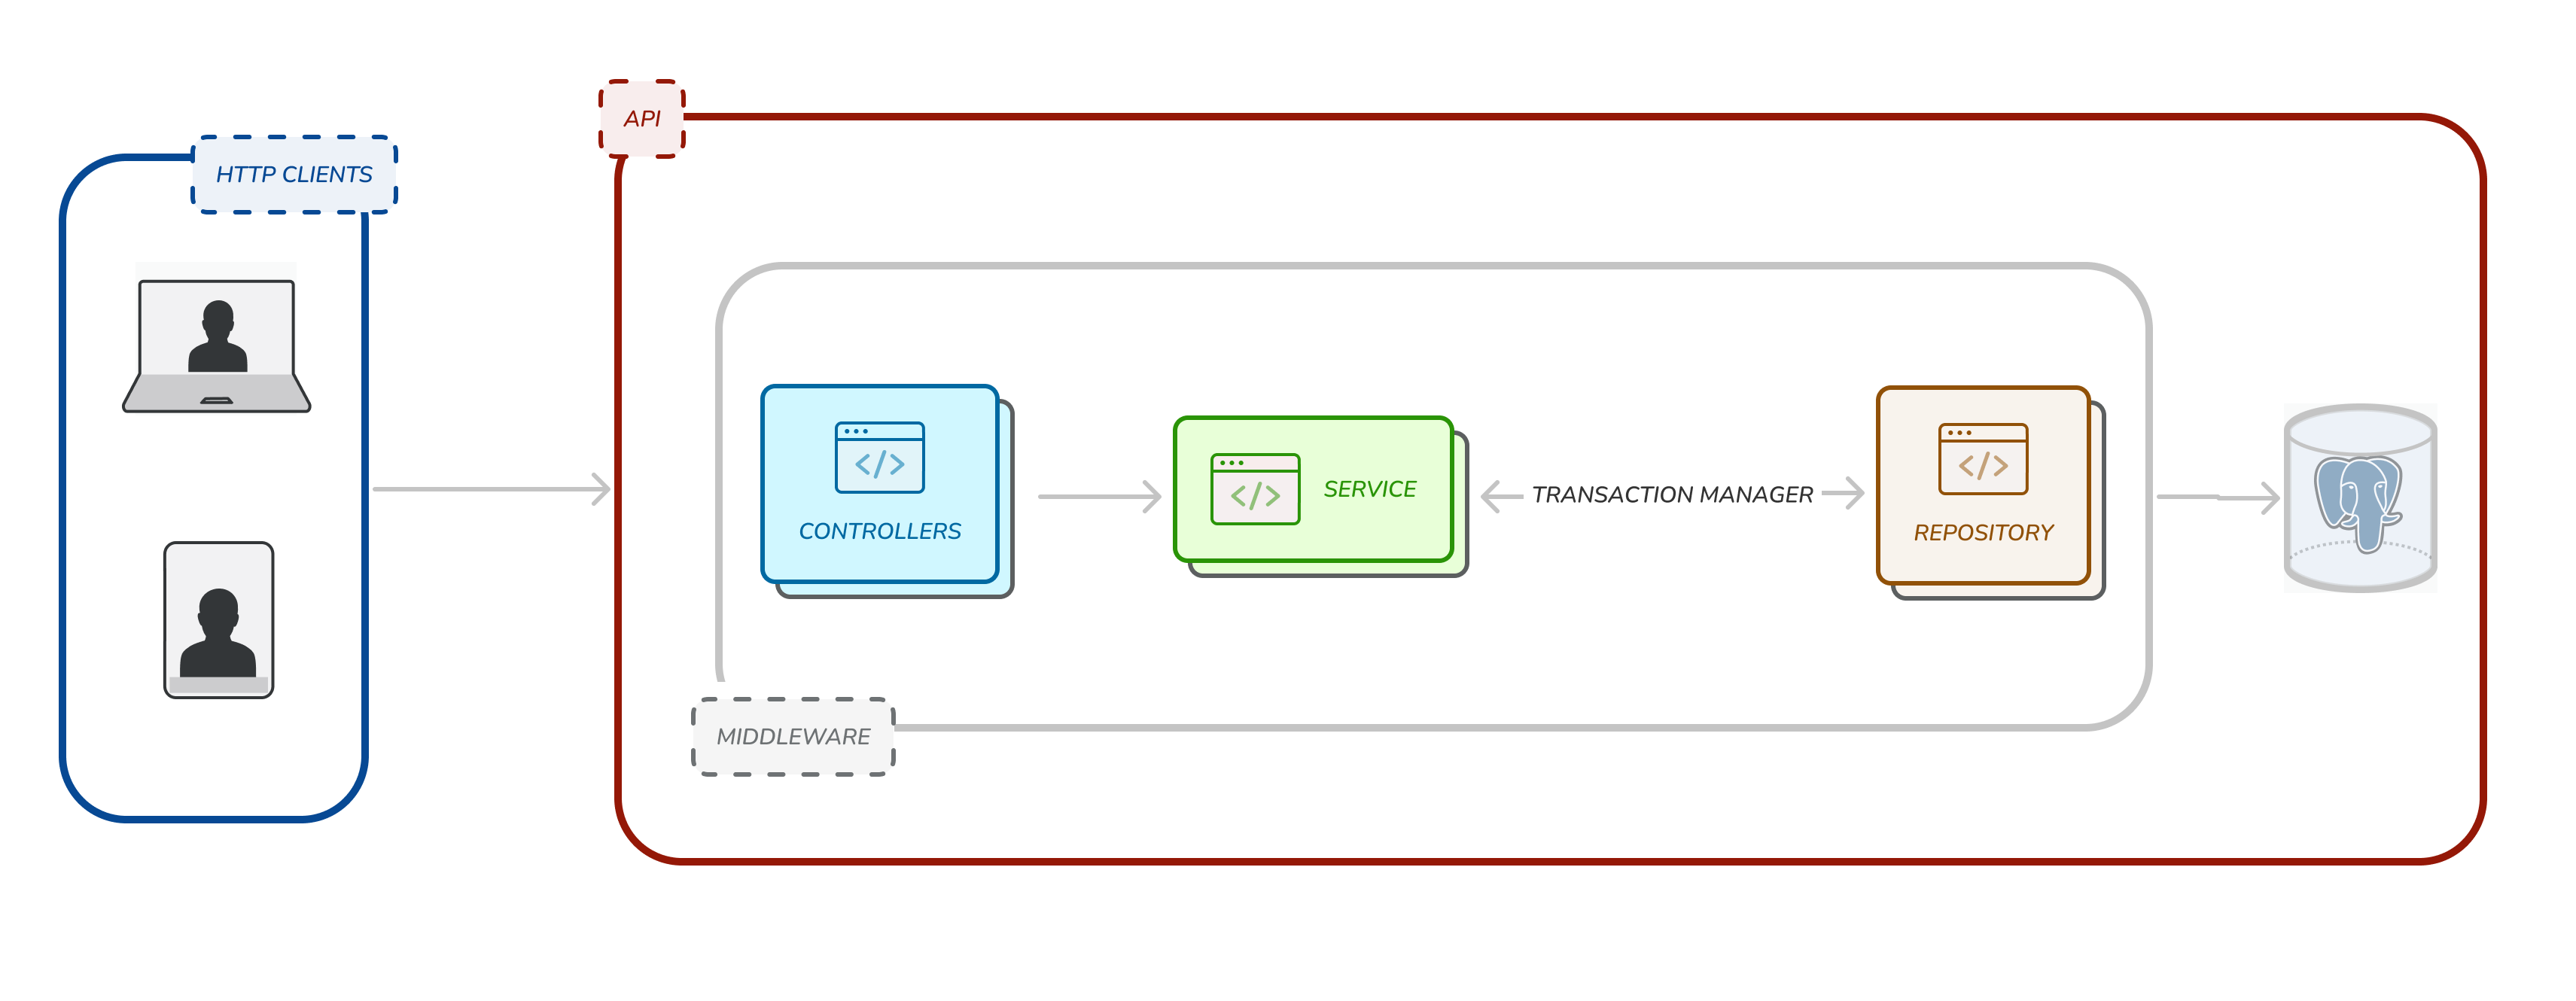
\includegraphics[width=1.05\textwidth]{img/API_structure.png}
\caption{API Architecture Overview}
\label{fig:api-structure}
\end{figure}

\subsection{Design Principles and Patterns}

To ensure robustness in error management, our API adopts the Problem Details for HTTP APIs standard (RFC 9457) \cite{rfc9457}. This specification allows the backend to communicate errors through structured, consistent responses, replacing ambiguous exceptions with clear, machine-readable diagnostic information.

The backend is organized into distinct layers to promote maintainability, scalability, and a strict separation of concerns. This modular approach allows for the isolated development and evolution of different system components:

\begin{itemize}
\item \textbf{Controllers}: Act as the entry point, managing incoming HTTP requests and orchestrating the appropriate responses.
\item \textbf{Services}: Encapsulate the core business logic, ensuring that domain rules are applied independently of the presentation layer.
\item \textbf{Repositories}: Define the data access layer, abstracting database interactions and shielding the business logic from persistence-specific details.
\end{itemize}

Furthermore, to uphold data consistency and integrity across complex operations, we implemented a \textbf{Transaction Manager}. This component ensures the atomicity of database interactions by grouping multiple operations into a single logical unit. Consequently, all operations within a transaction are committed only if entirely successful; otherwise, the system triggers a rollback, effectively preventing the database from entering an inconsistent state.

\subsection{Authentication and Authorization Interceptors}

To enforce security across our API, most endpoints are protected by an interception mechanism that validates not only user authentication but also the status of their account. Specifically, our system requires that every request originates from an authenticated user who has successfully verified their email address.

To streamline this, we implemented an \texttt{AuthenticatedUser} class that serves as a specialized parameter in controller actions. When a method signature includes this parameter, our interceptor system automatically triggers, performing a two-fold validation:
\begin{enumerate}
\item It verifies the integrity and validity of the authentication token or cookie provided in the request.
\item It confirms the user’s account status, ensuring that their email address has been verified.
\end{enumerate}

If either validation fails—whether the credentials are invalid or the email remains unconfirmed—the interceptor intercepts the execution flow and returns an appropriate error response following the Problem Details format, preventing the controller logic from ever being reached.

This design offers several architectural advantages:
\begin{itemize}
\item \textbf{Centralized Logic}: Authentication and authorization rules are consolidated within a single component, eliminating code duplication across controllers.
\item \textbf{Separation of Concerns}: Controller actions remain strictly focused on business logic, decoupled from security or identity verification.
\item \textbf{Declarative Security}: Security requirements are explicitly declared through method signatures, making the codebase easier to audit.
\item \textbf{Unified Mechanism}: The same interception pipeline transparently supports both token-based (mobile) and cookie-based (web) authentication.
\end{itemize}

Figure~\ref{fig:interceptor-functioning} illustrates the operational flow of this mechanism. When credentials are valid and the user is verified, the \texttt{AuthenticatedUser} object is populated with the user’s identity, allowing the request to proceed. Otherwise, the request is rejected with a descriptive error response, ensuring the system remains protected.

\begin{figure}[H]
\centering
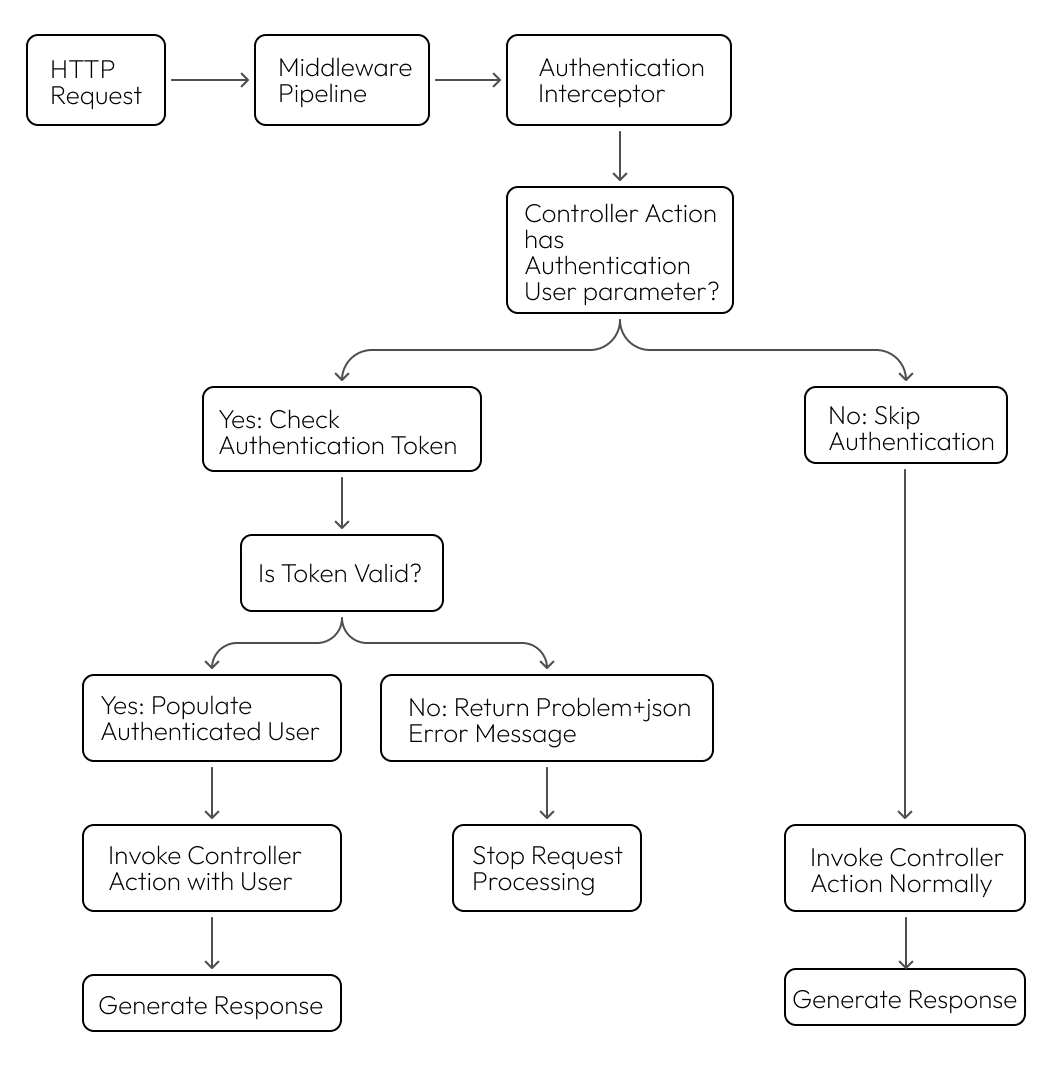
\includegraphics[width=10cm]{img/interceptor_functioning.png}
\caption{Authentication Interceptor Workflow}
\label{fig:interceptor-functioning}
\end{figure}

This pattern ensures a clean, maintainable, and highly secure boundary between security enforcement and business operations.

\subsection{Error Handling Middleware}

A cornerstone of our error management strategy is the global error-handling middleware, which serves as a protective layer between the core application logic and the client-side response. This component is designed to ensure that unexpected faults are captured and communicated in a standardized, predictable manner.

\begin{lstlisting}[caption={Error Handling Middleware Implementation}, label={lst:error-handling-middleware}]
private static async Task HandleExceptionAsync(HttpContext context, Exception exception)
{
var statusCode = (int)HttpStatusCode.InternalServerError;
context.Response.ContentType = "application/problem+json";
context.Response.StatusCode = statusCode;

    var problem = ProblemResponse.InternalServerError;

    var json = JsonSerializer.Serialize(problem);
    await context.Response.WriteAsync(json);
}
\end{lstlisting}

As illustrated in Listing~\ref{lst:error-handling-middleware}, this middleware fulfills two primary architectural roles:

\begin{itemize}
\item \textbf{Global Exception Interception}: It acts as a safety net, capturing any unhandled exceptions during request execution—such as database connectivity issues or unforeseen system failures. By intercepting these faults, the middleware prevents raw or sensitive stack trace information from propagating to the client, which significantly hardens the API against information disclosure.

\item \textbf{Standardized Response Mapping}: The middleware transforms intercepted exceptions into well-defined responses conforming to the \texttt{application/problem+json} format (RFC 9457). This ensures that error reporting remains consistent across the entire system, providing clients with a reliable and easily consumable interface for handling failures.
\end{itemize}

Technically, the implementation enforces a 500 Internal Server Error status code by default for unhandled faults. It then serializes a predefined ProblemResponse object into JSON, ensuring the output adheres strictly to our established API error contract, thereby maintaining seamless communication with the frontend.


\subsection{Email Service}

The system incorporates a dedicated email service primarily to orchestrate user identity verification. By requiring users to validate their registration via a unique verification code, we significantly enhance platform security and ensure that all accounts are linked to accessible, legitimate email addresses.

The verification workflow operates as follows:
\begin{itemize}
\item \textbf{Token Generation}: Upon registration, the system automatically generates a unique, time-sensitive verification code.
\item \textbf{Secure Dispatch}: The email service transmits this code to the user's provided email address.
\item \textbf{Identity Confirmation}: The user is required to input the received code within the application to finalize the account activation process.
\end{itemize}

Figure~\ref{fig:email-service-structure} illustrates the internal architecture of the email service and its integration with the core system components.

\begin{figure}[H]
\centering
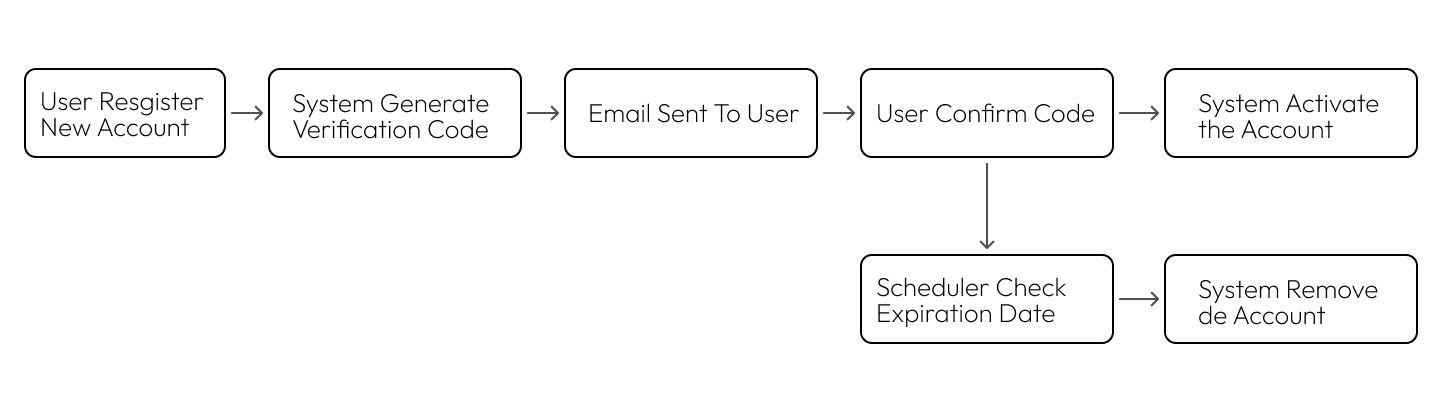
\includegraphics[width=1.05\textwidth]{img/email_service_structure.png}
\caption{Email Service Architectural Overview}
\label{fig:email-service-structure}
\end{figure}

By maintaining this structured approach to identity verification, the email service serves as a cornerstone for maintaining a clean and trustworthy user base within the application ecosystem.

\subsection{Authentication Pipeline}

To ensure that only authorized users can access protected resources, we implemented a robust authentication pipeline. This mechanism is responsible for validating user credentials and account status before any business logic is executed within the controller actions.

Architecture of the Authentication Pipeline
The authentication process is enforced through a custom filter, RequireAuthenticationAttribute, which integrates into the ASP.NET Core request lifecycle. This attribute works in conjunction with a TokenProcessor service, forming a centralized validation pipeline:

\begin{enumerate}
\item \textbf{Identity Resolution}: The pipeline retrieves the authentication token either from the request headers or the application cookies.
\item \textbf{Token Validation and Identity Mapping}: The TokenProcessor validates the token and resolves the user's identity, ensuring that the session is active and legitimate.
\item \textbf{Authorization and Account Status Check}: Beyond verifying the token, the pipeline explicitly checks the \texttt{IsEmailConfirmed} flag. If the account is not verified, the system terminates the request and returns a \texttt{403 Forbidden} status, mandating email confirmation to proceed.
\item \textbf{Dependency Injection}: Once the user is authenticated and verified, the pipeline populates the \texttt{HttpContext.Items} with an \texttt{AuthenticatedUser} object. This object is then automatically injected into controller actions via a custom AuthenticatedUserModelBinder, allowing for clean and declarative parameter access.
\end{enumerate}

Cookie Configuration and Security
For web-based interactions, the application utilizes secure cookie-based session management. Listing~\ref{lst:login-response} illustrates the configuration used to persist the authentication session:

\begin{lstlisting}[caption={Authentication Cookie Configuration}, label={lst:login-response}]
var cookieOptions = new CookieOptions
{
HttpOnly = true,
Secure = false, // Must be true in production
SameSite = SameSiteMode.Strict,
Expires = DateTime.Now.AddDays(7)
};
Response.Cookies.Append("token", tokenValue, cookieOptions);
\end{lstlisting}

This configuration adheres to security best practices:
\begin{itemize}
\item \textbf{HttpOnly}: Renders the cookie inaccessible to client-side scripts, effectively preventing Cross-Site Scripting (XSS) attacks.
\item \textbf{SameSite (Strict)}: Instructs the browser to only send the cookie with requests originating from our domain, providing a robust defense against Cross-Site Request Forgery (CSRF).
\item \textbf{Expiration Policy}: Sets a persistent 7-day session, which is dynamically maintained and refreshed upon valid user interaction.
\end{itemize}

By decoupling security validation from business logic through this custom pipeline, we ensure that authentication requirements are explicitly declared via method signatures, resulting in a cleaner, more secure, and highly maintainable codebase.